\section{Misurazione e aggiornamento adattivo dei profili energetici}
\label{sec:worker}

Una volta introdotto il modello di funzione logica con varianti multiple,
è necessario dotare il sistema di un meccanismo capace di aggiornare
dinamicamente i profili energetici sulla base dei consumi effettivamente
osservati a runtime. Un approccio statico, in cui il costo energetico di
una variante viene stimato offline e rimane invariato nel tempo, risulta
inadeguato in contesti di esecuzione reali: il consumo energetico di un
container è influenzato da fattori mutevoli quali il carico del nodo,
le interferenze tra istanze concorrenti e le variazioni dinamiche della
frequenza di CPU.

La soluzione adottata è un \emph{feedback loop} periodico che trasforma
il profilo energetico in una grandezza adattiva, aggiornata continuamente
in funzione del contesto di esecuzione. Il componente responsabile è un
worker di raccolta eseguito in background, illustrato in
Figura~\ref{fig:worker-architecture}.

\begin{figure}[ht]
    \centering
    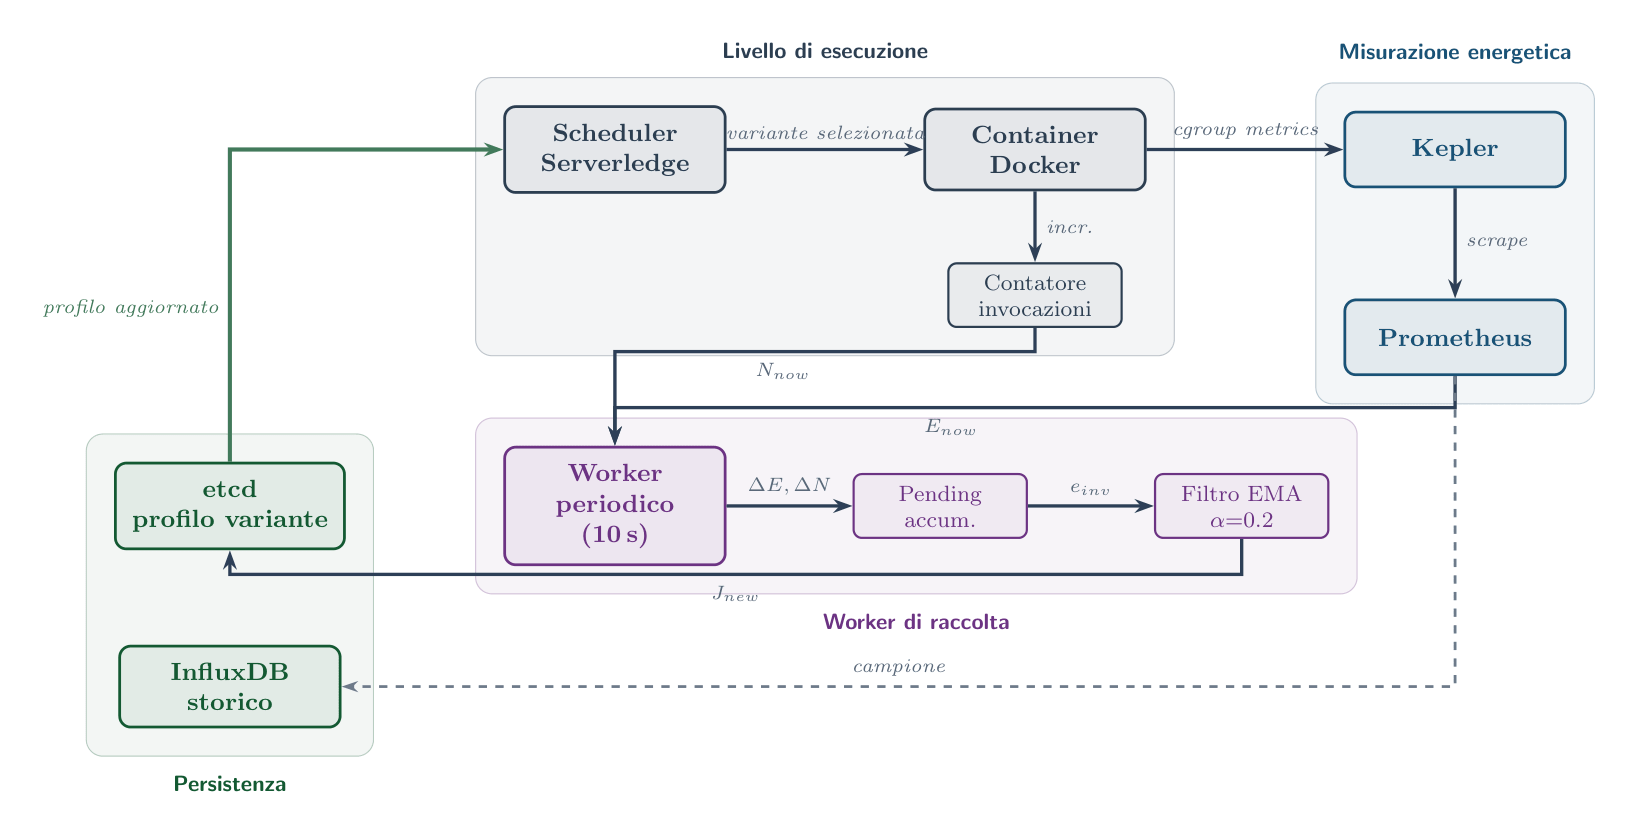
\includegraphics[width=\textwidth]{figures/Worker.png}
    \caption{Schema del feedback loop energetico. Il worker periodico
    legge le metriche cumulative da Kepler tramite Prometheus e il numero
    di invocazioni dal contatore locale, calcola i delta, applica un
    filtro EMA e aggiorna il profilo persistito in etcd, archiviando
    contestualmente i campioni in InfluxDB.}
    \label{fig:worker-architecture}
\end{figure}


\subsection{Tracciamento dei container e conteggio delle invocazioni}
\label{subsec:container-registry}

Per attribuire correttamente il consumo energetico alle singole varianti,
il sistema deve mantenere una corrispondenza stabile tra i container
Docker attivi e le funzioni in esecuzione. A tal fine il package
\texttt{energy} mantiene un registro in memoria che associa a ciascun
container una struttura \texttt{ContainerState} contenente:

\begin{itemize}
    \item l'identificatore del container (\texttt{ContainerID});
    \item il nome interno della variante (\texttt{FunctionName}), il
    \texttt{LogicalName} e il \texttt{VariantID};
    \item i valori di baseline dell'energia cumulativa e del numero di
    invocazioni (\texttt{LastJoule}, \texttt{LastInvocations}),
    impiegati per il calcolo dei delta incrementali;
    \item gli accumulatori \texttt{PendingEnergyJ} e
    \texttt{PendingInvocations}, necessari per gestire il disallineamento
    temporale tra metriche energetiche e contatori locali.
\end{itemize}

La registrazione avviene sia alla creazione del container sia, in modo
difensivo, al momento dell'invocazione, così da gestire correttamente il
caso di \emph{warm start}. Se un container è già presente nel registro,
la sua identità (mapping container-variante) non viene modificata,
garantendo coerenza per l'intero ciclo di vita del container.

Parallelamente, viene mantenuto un contatore atomico di invocazioni per
container, incrementato al completamento di ogni richiesta.

\subsection{Il worker periodico di raccolta}
\label{subsec:worker-periodico}

Il worker è implementato come una goroutine avviata all'inizializzazione
della piattaforma. Con cadenza di 10 secondi, esegue un ciclo di raccolta
(\texttt{Collect}) operando su uno snapshot thread-safe del
\texttt{ContainerRegistry}, in modo da isolare la lettura dallo stato
condiviso senza bloccare le operazioni concorrenti.

Per ciascun container attivo vengono acquisiti:

\begin{itemize}
    \item il valore cumulativo di energia $E_{now}$, esposto da Kepler e
    reso disponibile tramite l'endpoint Prometheus;
    \item il numero cumulativo di invocazioni $N_{now}$, mantenuto
    aggiornato dal contatore locale.
\end{itemize}

Vengono quindi calcolati i delta rispetto all'osservazione precedente:

\begin{equation}
    \Delta E = E_{now} - E_{last}
    \qquad
    \Delta N = N_{now} - N_{last}
\end{equation}

La presenza di valori negativi segnala un reset del container o del
contatore, condizione possibile ad esempio in seguito a un riavvio
dell'istanza, e comporta la reinizializzazione delle variabili senza
produzione di campioni, evitando attribuzioni energetiche errate.


\subsection{Attribuzione dell'energia per invocazione e gestione del lag}
\label{subsec:lag}

Le metriche esposte da Kepler hanno natura cumulativa e sono soggette a
un ritardo di campionamento intrinseco al ciclo di scraping di Prometheus.
Il contatore locale di invocazioni, al contrario, viene aggiornato
immediatamente al termine di ogni esecuzione. Può quindi verificarsi la
condizione:

\[
    \Delta N > 0 \quad \text{e} \quad \Delta E = 0
\]

in cui nuove invocazioni sono già state completate ma il relativo consumo
energetico non è ancora riflesso nella metrica cumulativa. Calcolare in
questo caso il consumo medio per invocazione produrrebbe una sottostima
sistematica.

Per gestire questo disallineamento, i delta vengono accumulati nei
campi \texttt{PendingEnergyJ} e \texttt{PendingInvocations}. L'attribuzione
effettiva avviene solo quando entrambi gli accumulatori risultano positivi,
garantendo che l'energia osservata e il numero di esecuzioni considerate
siano coerenti tra loro:

\begin{equation}
    e_{inv} = \frac{E_{pending}}{N_{pending}}
\end{equation}

Il valore $e_{inv}$ rappresenta la stima istantanea del consumo medio
per invocazione nel periodo considerato e costituisce l'ingresso per la
fase di aggiornamento adattivo del profilo.


\subsection{Aggiornamento del profilo tramite media mobile esponenziale}
\label{subsec:ema}

La stima istantanea $e_{inv}$ può essere affetta da rumore dovuto a
interferenze tra container, variazioni dinamiche della frequenza di CPU
o fluttuazioni del carico di sistema. Applicare direttamente tale valore
al profilo energetico potrebbe causare oscillazioni indesiderate nelle
decisioni dello scheduler.

Per stabilizzare la stima viene applicata una \emph{Exponential Moving
Average} (EMA):

\begin{equation}
    J_{new} = \alpha \cdot e_{inv} + (1 - \alpha) \cdot J_{old}
\end{equation}

con $\alpha = 0.2$. Il parametro $\alpha$ governa il compromesso tra
due esigenze contrastanti:

\begin{itemize}
    \item \textbf{Reattività}: valori elevati rendono il profilo
    rapidamente adattabile a variazioni strutturali del consumo energetico;
    \item \textbf{Stabilità}: valori ridotti attenuano il contributo
    di singoli campioni anomali, producendo una stima più robusta.
\end{itemize}

La scelta di $\alpha = 0.2$ rappresenta un equilibrio empirico: il
sistema filtra efficacemente i picchi transitori, mantenendo al
contempo una capacità di adattamento progressivo al nuovo regime
energetico nell'arco di circa $1/\alpha$ cicli di aggiornamento,
corrispondenti a circa 50 secondi con la cadenza attuale del worker.

Il valore aggiornato $J_{new}$ viene scritto nel campo
\texttt{InvocationJoule} della variante corrispondente e persistito in
etcd, rendendolo immediatamente disponibile allo scheduler per le
decisioni di selezione successive.



\subsection{Archiviazione su InfluxDB}
\label{subsec:influxdb}

Contestualmente all'aggiornamento in etcd, ogni campione viene archiviato
in InfluxDB come punto della \emph{measurement} \texttt{energy\_sample},
con tag \texttt{container\_id}, \texttt{logical\_name},
\texttt{function\_name}, \texttt{variant\_id} e campo
\texttt{invocation\_joule}.

La separazione tra i due store riflette le loro funzioni distinte: etcd
fornisce allo scheduler la stima corrente con latenza minima; InfluxDB
preserva la serie storica dei campioni, che costituisce la base
statistica per il meccanismo di esplorazione descritto nella
Sezione~\ref{sec:esplorazione-ucb}.